\documentclass{article}
\usepackage{amsmath}
\usepackage{geometry}
\usepackage{listings}
\usepackage{fancyvrb}
\usepackage{multicol}
\usepackage{graphicx}
\usepackage{caption}
\usepackage{tikz}
\usepackage{eso-pic}
\usepackage{array}
\usepackage{afterpage}

\geometry{a4paper, left=0.75in, right=0.75in, top=0.65in, bottom=0.25in}
\pagestyle{empty}
\pagenumbering{gobble}

% Define the border and header drawing command
\newcommand\PageBorder{%
  \begin{tikzpicture}[remember picture,overlay]
    % Date Label (top left)
    \node[anchor=north west, font=\large] 
      at ([xshift=0.75in,yshift=-0.25in]current page.north west) {Date:\hspace{3cm}};
    % Page No Label (top right)
    \node[anchor=north east, font=\large] 
      at ([xshift=-1.25in,yshift=-0.25in]current page.north east) {Page No:\hspace{2.5cm}};
  \end{tikzpicture}% % <-- pushes text down
}
\AddToShipoutPicture{\PageBorder}

%dont edit anything above............


\begin{document}
\section*{\centering{Cycle 1}}
\begin{figure}[h!]
    \centering
    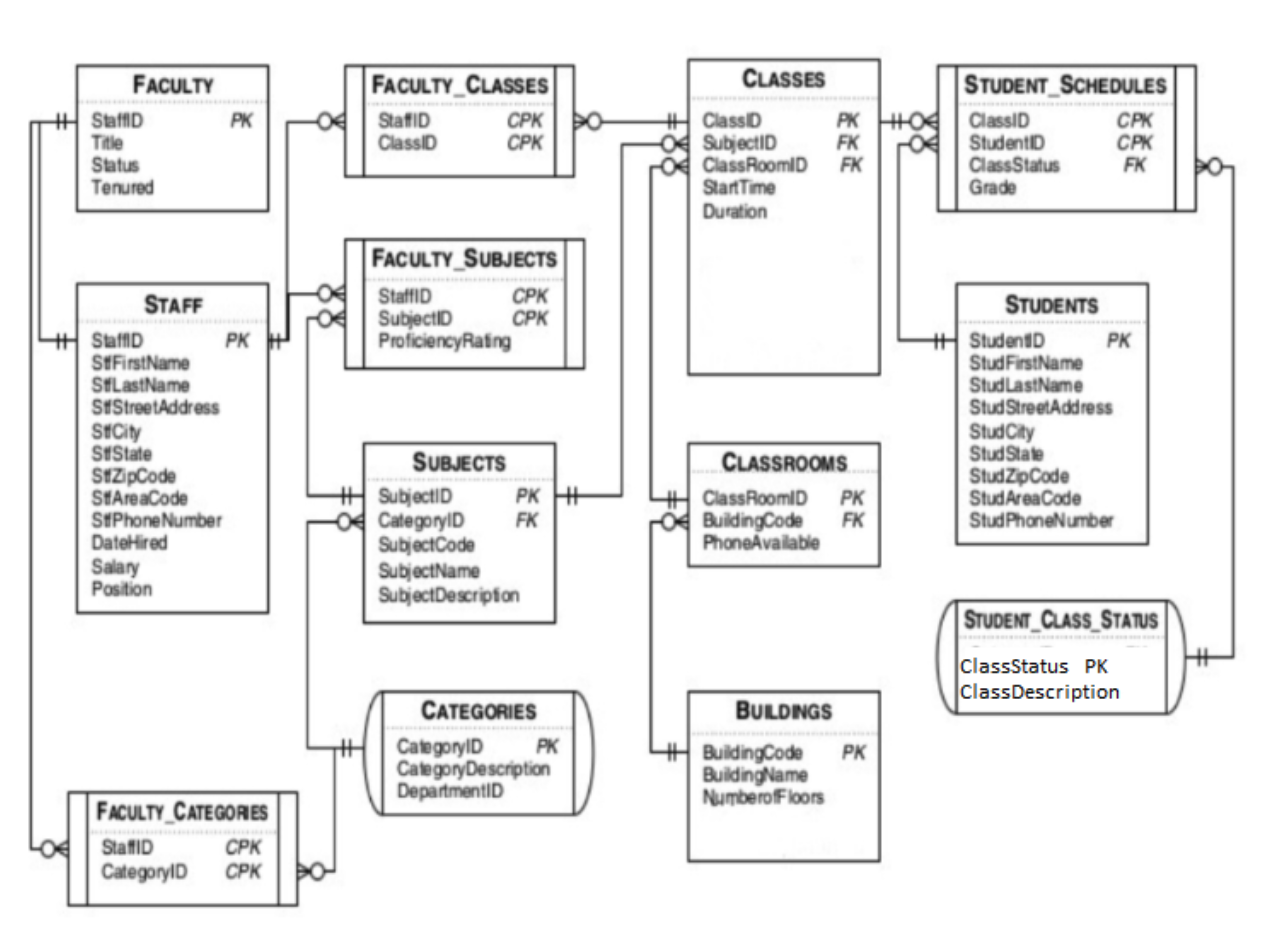
\includegraphics[width=0.95\textwidth]{./uml_diagram.png} % Replace with the fig in the cycle
    \label{fig:schema}
\end{figure}
\subsection*{1.  Design the ER diagram from the given schema.}
\begin{figure}[h!]
    \centering
    \includegraphics[width=0.75\textwidth]{./er_diagram.png} %er diagram image
    \label{fig:schema}
\end{figure}
\\
\newpage
\subsection*{2. Create the database with proper tables, columns, column types and \\
constraints.}

\subsubsection*{Staff Table}
Query:
\begin{Verbatim}[frame=single,framerule=1pt,fontfamily=courier,fontsize=\small]
CREATE TABLE staff (
    staffID bigint GENERATED ALWAYS AS IDENTITY PRIMARY KEY,
    stfFirstName text,
    stfLastName text,
    stfStreetAdress text,
    stfCity text,
    stfState text,
    stfZipCode int,
    stfAreaCode int,
    stfPhoneNumber text,
    dateHired date,
    salary bigint,
    position text
);
\end{Verbatim}
\begin{figure}[h]
    \centering
    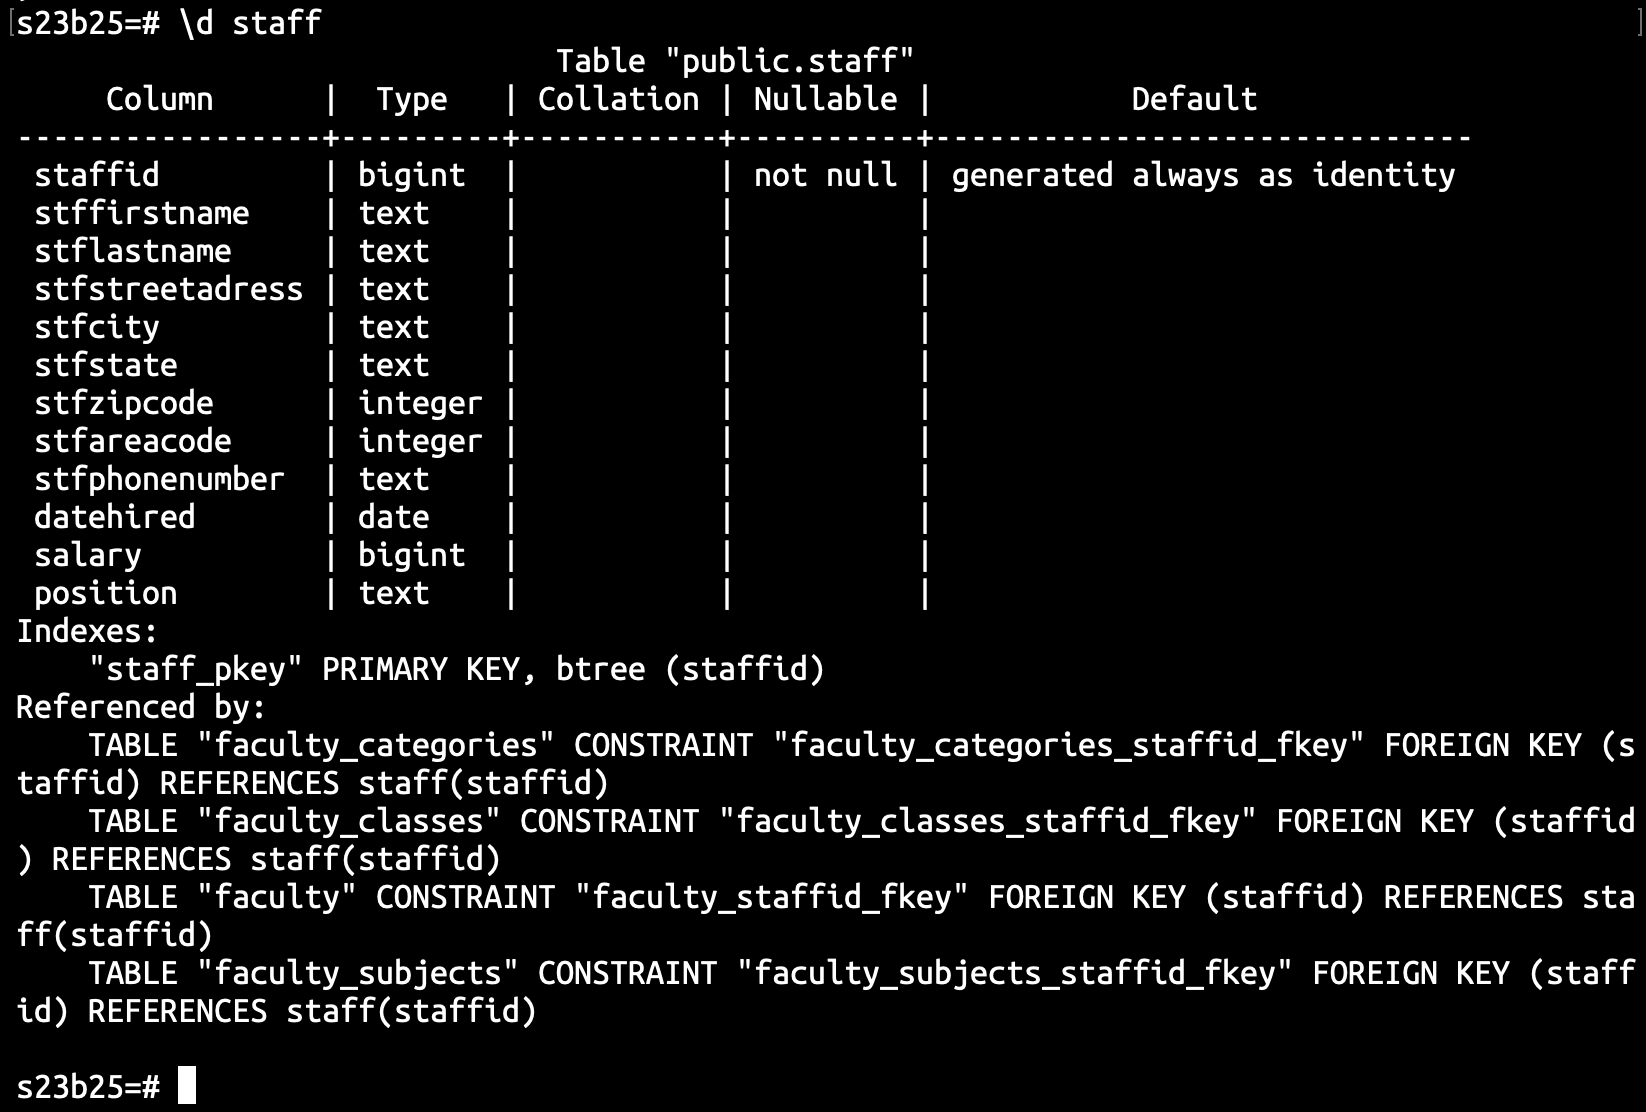
\includegraphics[width=\textwidth]{./o_1_staff.png}
\end{figure}

\subsubsection*{Faculty Table}
Query:
\begin{Verbatim}[frame=single,framerule=1pt,fontfamily=courier,fontsize=\small]
CREATE TABLE faculty(
    staffID bigint REFERENCES staff (staffID) UNIQUE NOT NULL,
    title text,
    status text,
    tenured date 
);
\end{Verbatim}
\begin{figure}[h]
    \centering
    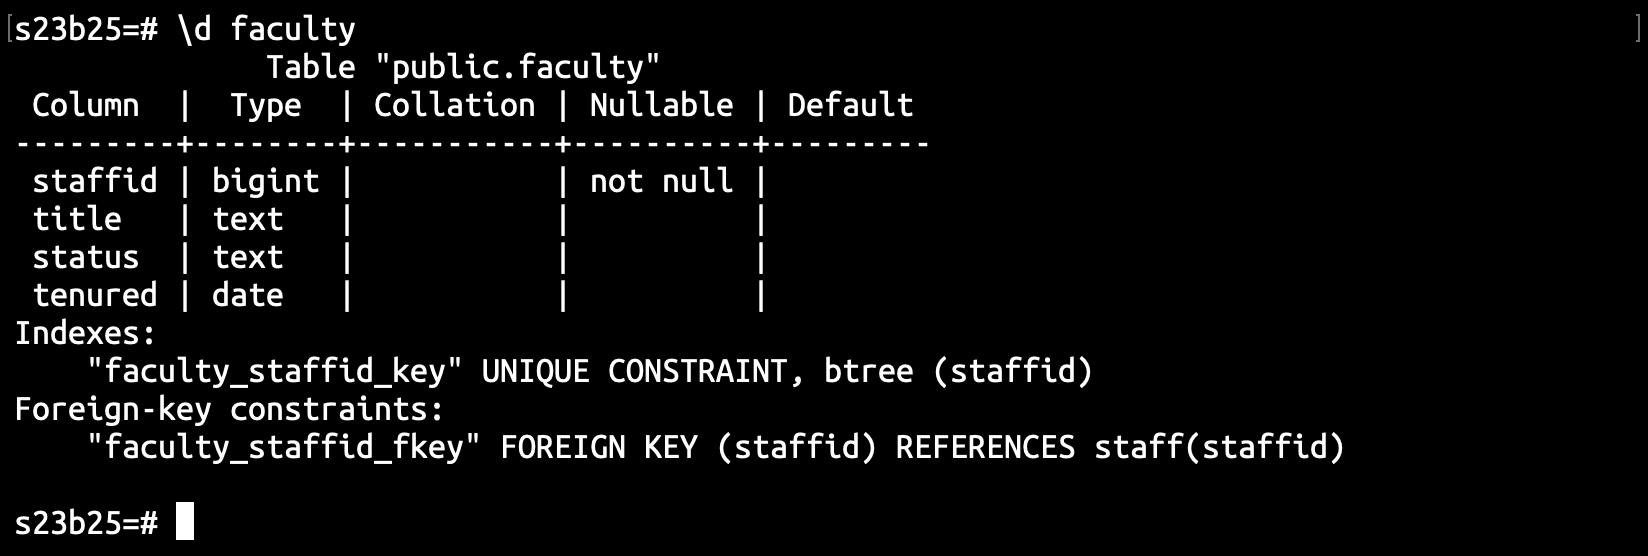
\includegraphics[width=\textwidth]{./o_2_faculty.png}
\end{figure}

\subsubsection*{Categories Table}
Query:
\begin{Verbatim}[frame=single,framerule=1pt,fontfamily=courier,fontsize=\small]
CREATE TABLE categories(
    categoryid bigint GENERATED ALWAYS AS IDENTITY PRIMARY KEY,
    categoryDescription text,
    departmentID bigint
);
\end{Verbatim}
\begin{figure}[h]
    \centering
    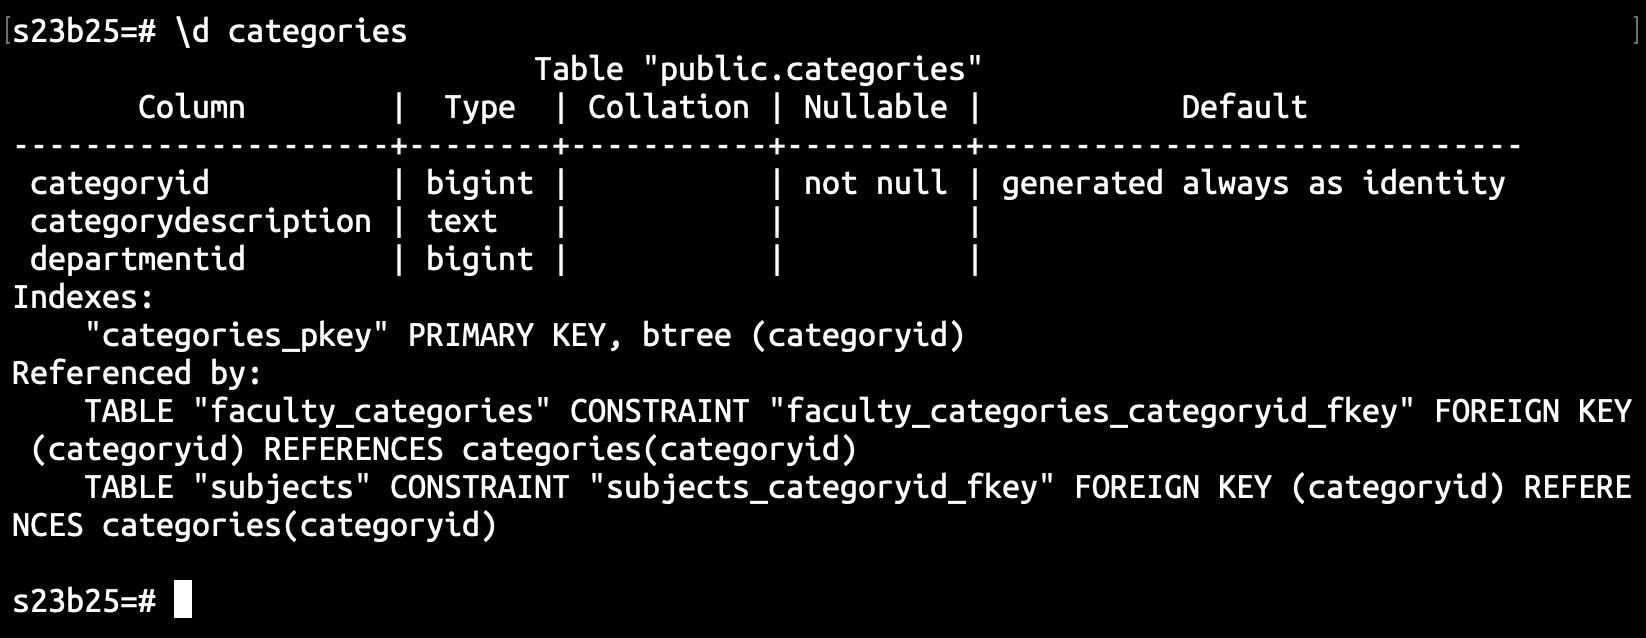
\includegraphics[width=\textwidth]{./o_3_categories.png}
\end{figure}

\subsubsection*{Faculty-Categories Table}
Query:
\begin{Verbatim}[frame=single,framerule=1pt,fontfamily=courier,fontsize=\small]
CREATE TABLE faculty_categories(
    staffID bigint REFERENCES staff (staffID),
    categoryID bigint REFERENCES categories (categoryID),
    PRIMARY KEY (staffID, categoryID)
);
\end{Verbatim}
\begin{figure}[h]
    \centering
    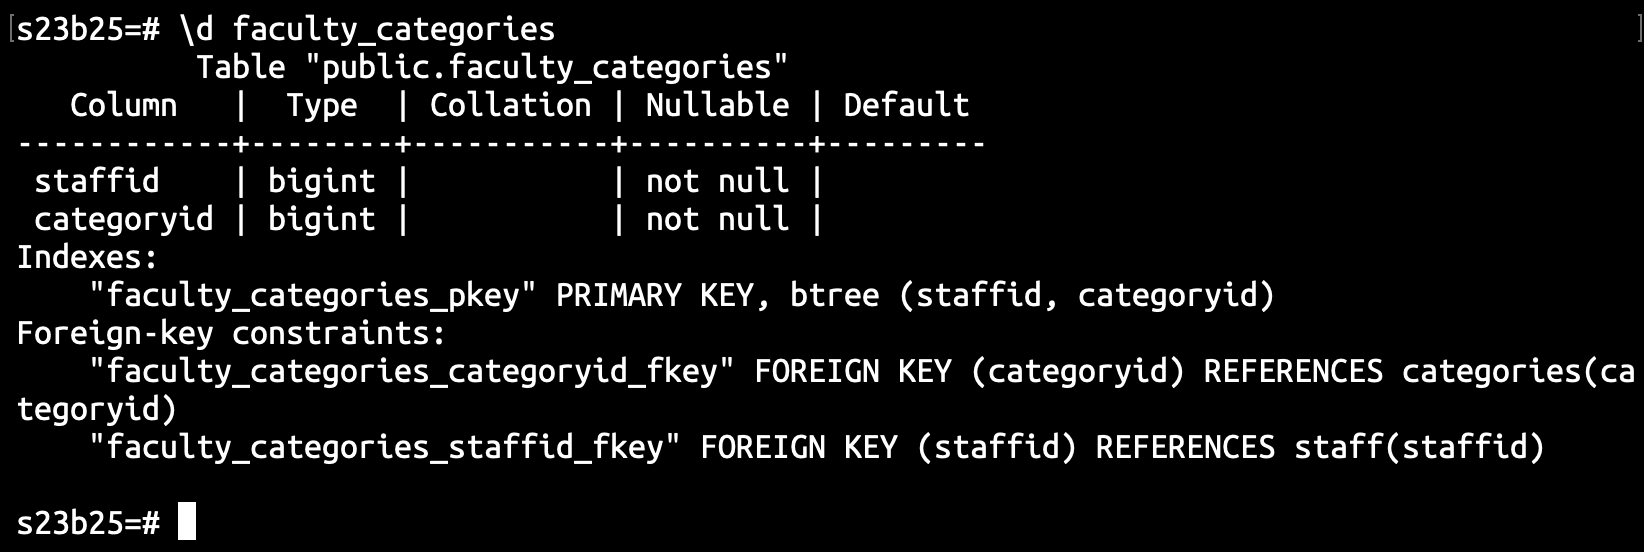
\includegraphics[width=\textwidth]{./o_4_faculty_categories.png}
\end{figure}

\subsubsection*{Subjects Table}
Query:
\begin{Verbatim}[frame=single,framerule=1pt,fontfamily=courier,fontsize=\small]
CREATE TABLE subjects(
    subjectID bigint GENERATED ALWAYS AS IDENTITY PRIMARY KEY,
    categoryID bigint REFERENCES categories (categoryID),
    subjectCode int,
    subjectName text,
    subjectDescription text
);
\end{Verbatim}
\begin{figure}[h]
    \centering
    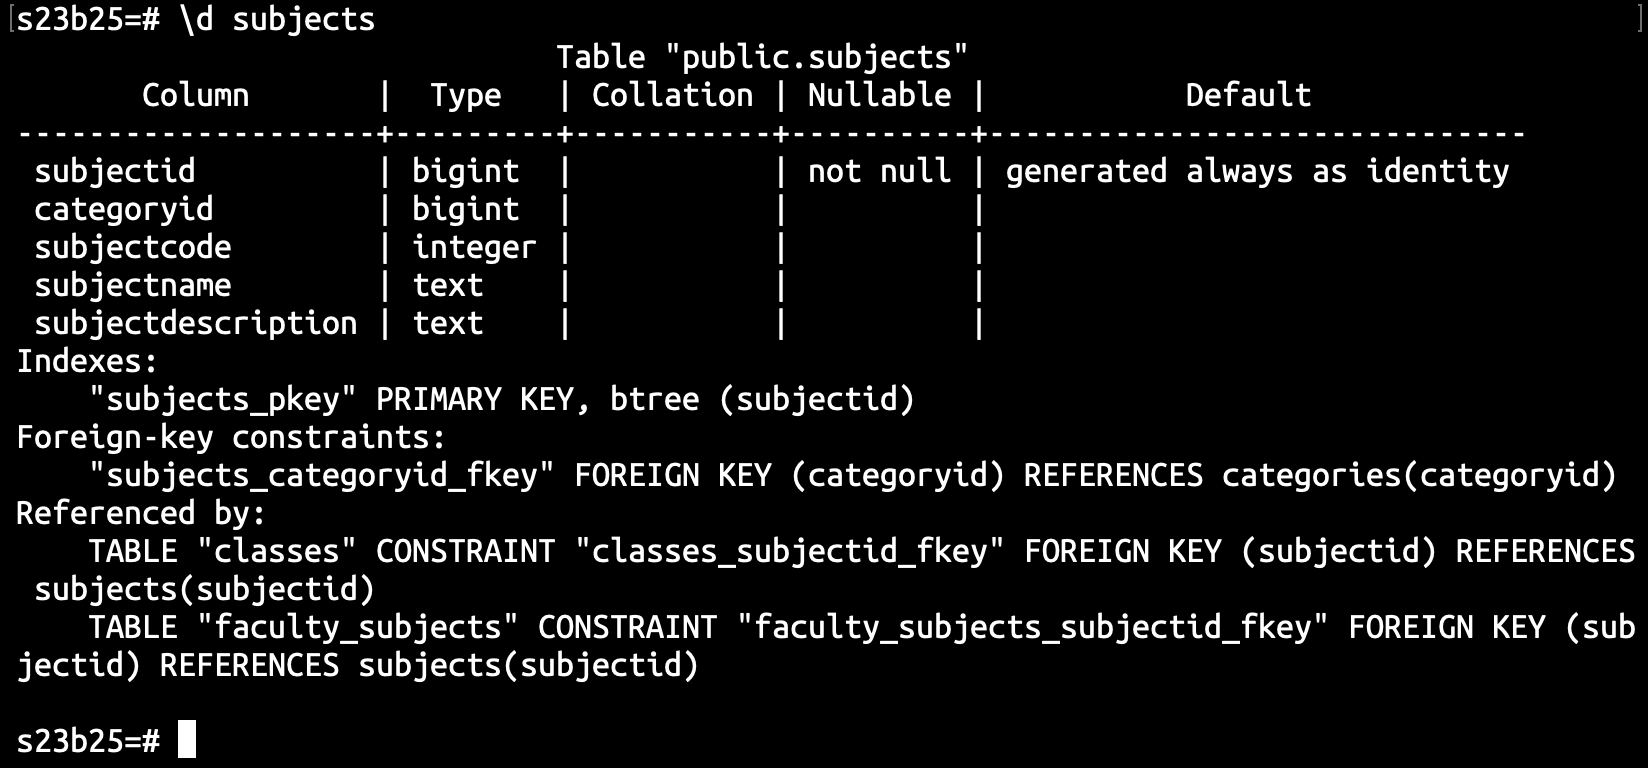
\includegraphics[width=\textwidth]{./o_5_subjects.png}
\end{figure}

\subsubsection*{Faculty-Subjects Table}
Query:
\begin{Verbatim}[frame=single,framerule=1pt,fontfamily=courier,fontsize=\small]
CREATE TABLE faculty_subjects(
    staffID bigint REFERENCES staff (staffID),
    subjectID bigint REFERENCES subjects (subjectID),
    proficiencyRating int,
    PRIMARY KEY (staffID, subjectID)
);
\end{Verbatim}
\begin{figure}[h]
    \centering
    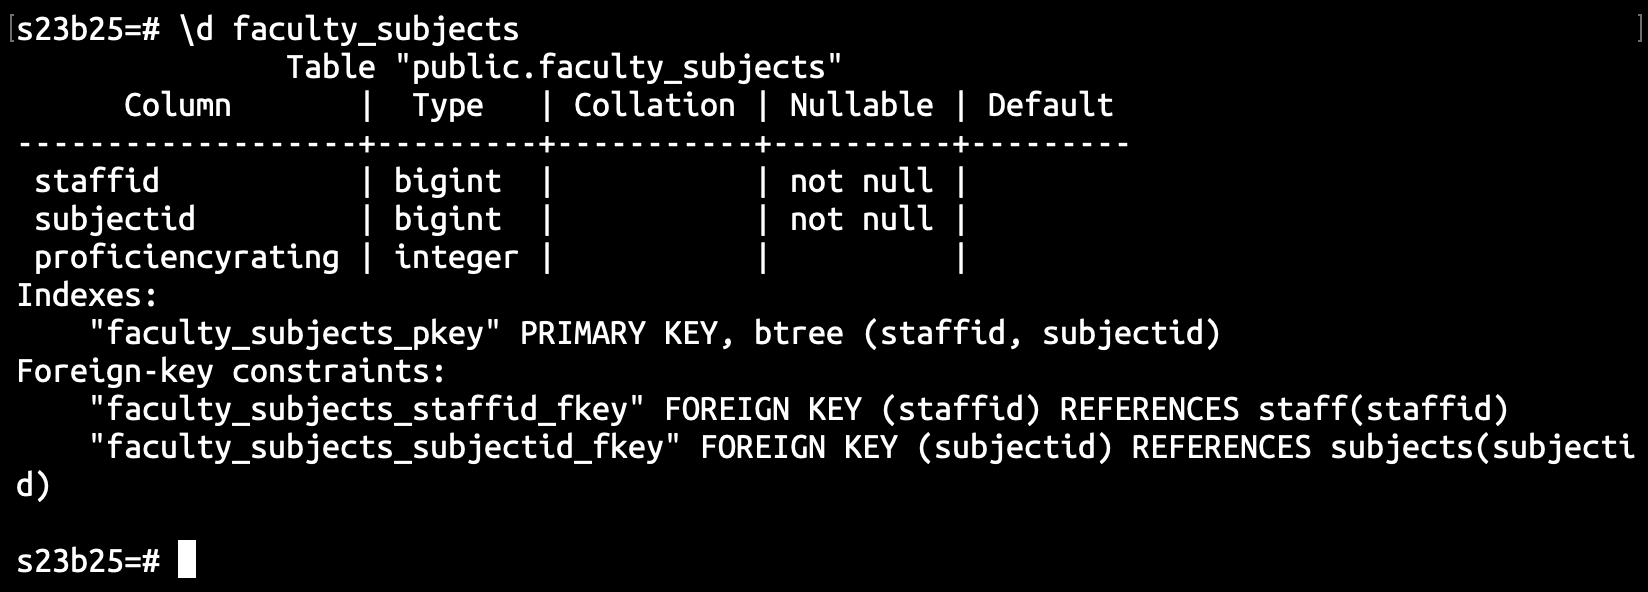
\includegraphics[width=\textwidth]{./o_6_faculty_subjects.png}
\end{figure}

\subsubsection*{Buildings Table}
Query:
\begin{Verbatim}[frame=single,framerule=1pt,fontfamily=courier,fontsize=\small]
CREATE TABLE buildings(
    buildingCode bigint GENERATED ALWAYS AS IDENTITY PRIMARY KEY,
    buildingName text,
    numberOfFloorts int
);
\end{Verbatim}
\begin{figure}[h]
    \centering
    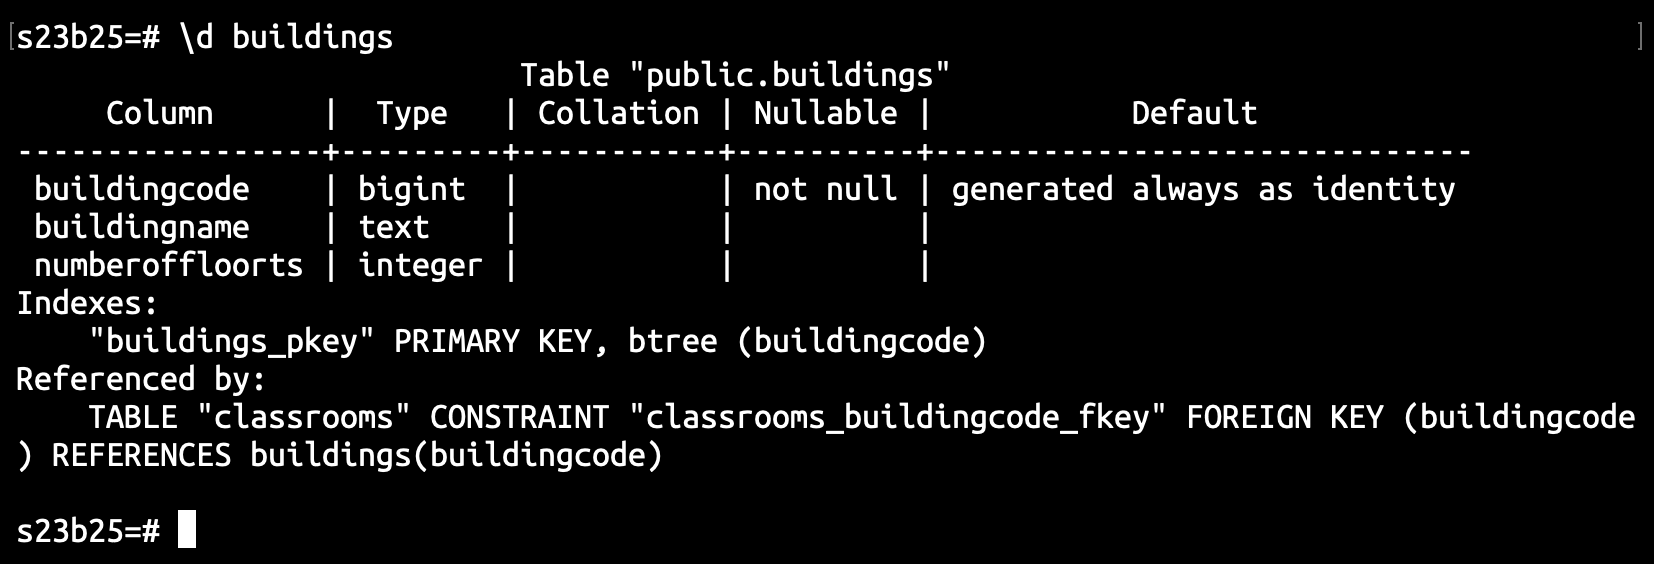
\includegraphics[width=\textwidth]{./o_7_buildings.png}
\end{figure}

\subsubsection*{Classrooms Table}
Query:
\begin{Verbatim}[frame=single,framerule=1pt,fontfamily=courier,fontsize=\small]
CREATE TABLE classrooms(
    classroomID bigint GENERATED ALWAYS AS IDENTITY PRIMARY KEY,
    buildingCode bigint REFERENCES buildings (buildingCode),
    phoneAvailable text
);
\end{Verbatim}
\begin{figure}[h]
    \centering
    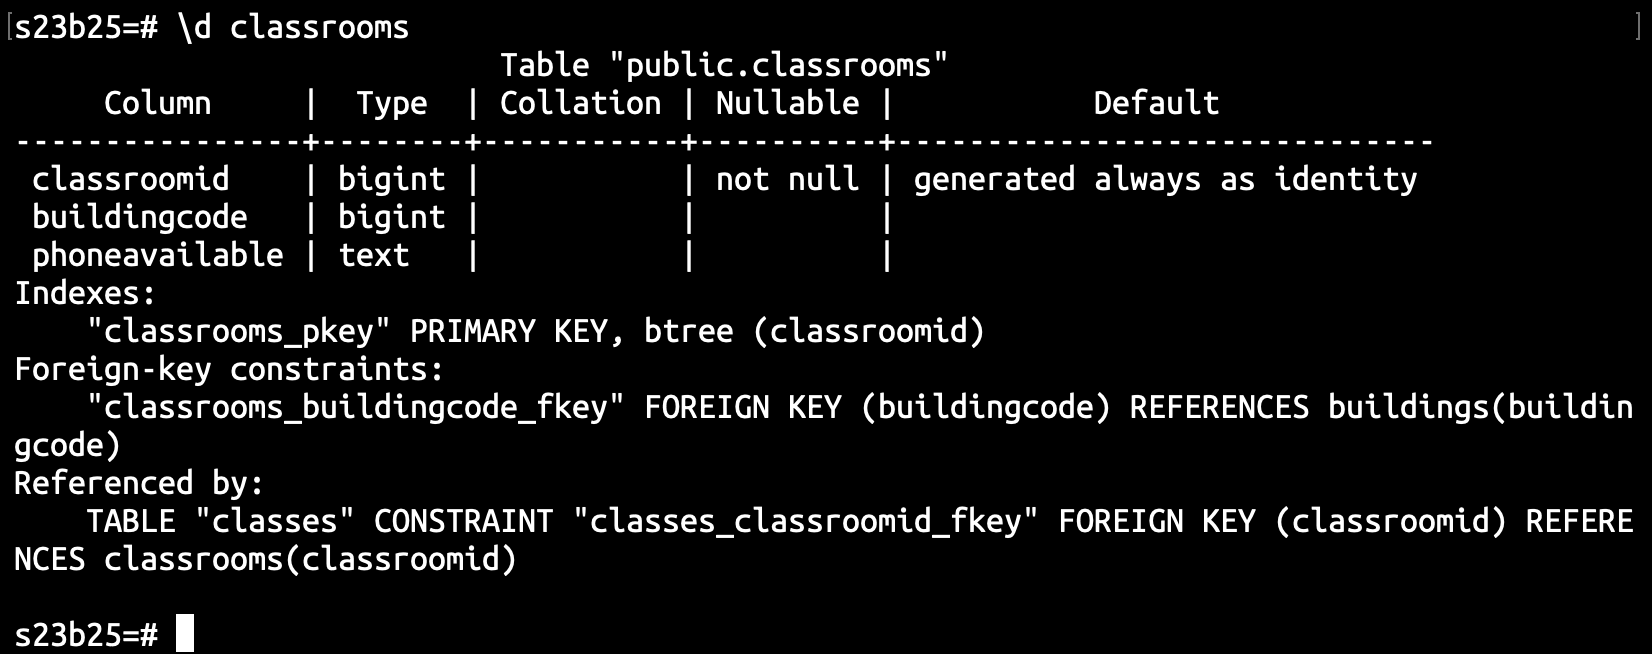
\includegraphics[width=\textwidth]{./o_8_classrooms.png}
\end{figure}

\subsubsection*{Classes Table}
Query:
\begin{Verbatim}[frame=single,framerule=1pt,fontfamily=courier,fontsize=\small]
CREATE TABLE classes(
    classID bigint GENERATED ALWAYS AS IDENTITY PRIMARY KEY,
    subjectID bigint REFERENCES subjects (subjectID),
    classroomID bigint REFERENCES classrooms (classroomID),
    startTime time,
    duration int
);
\end{Verbatim}
\begin{figure}[h]
    \centering
    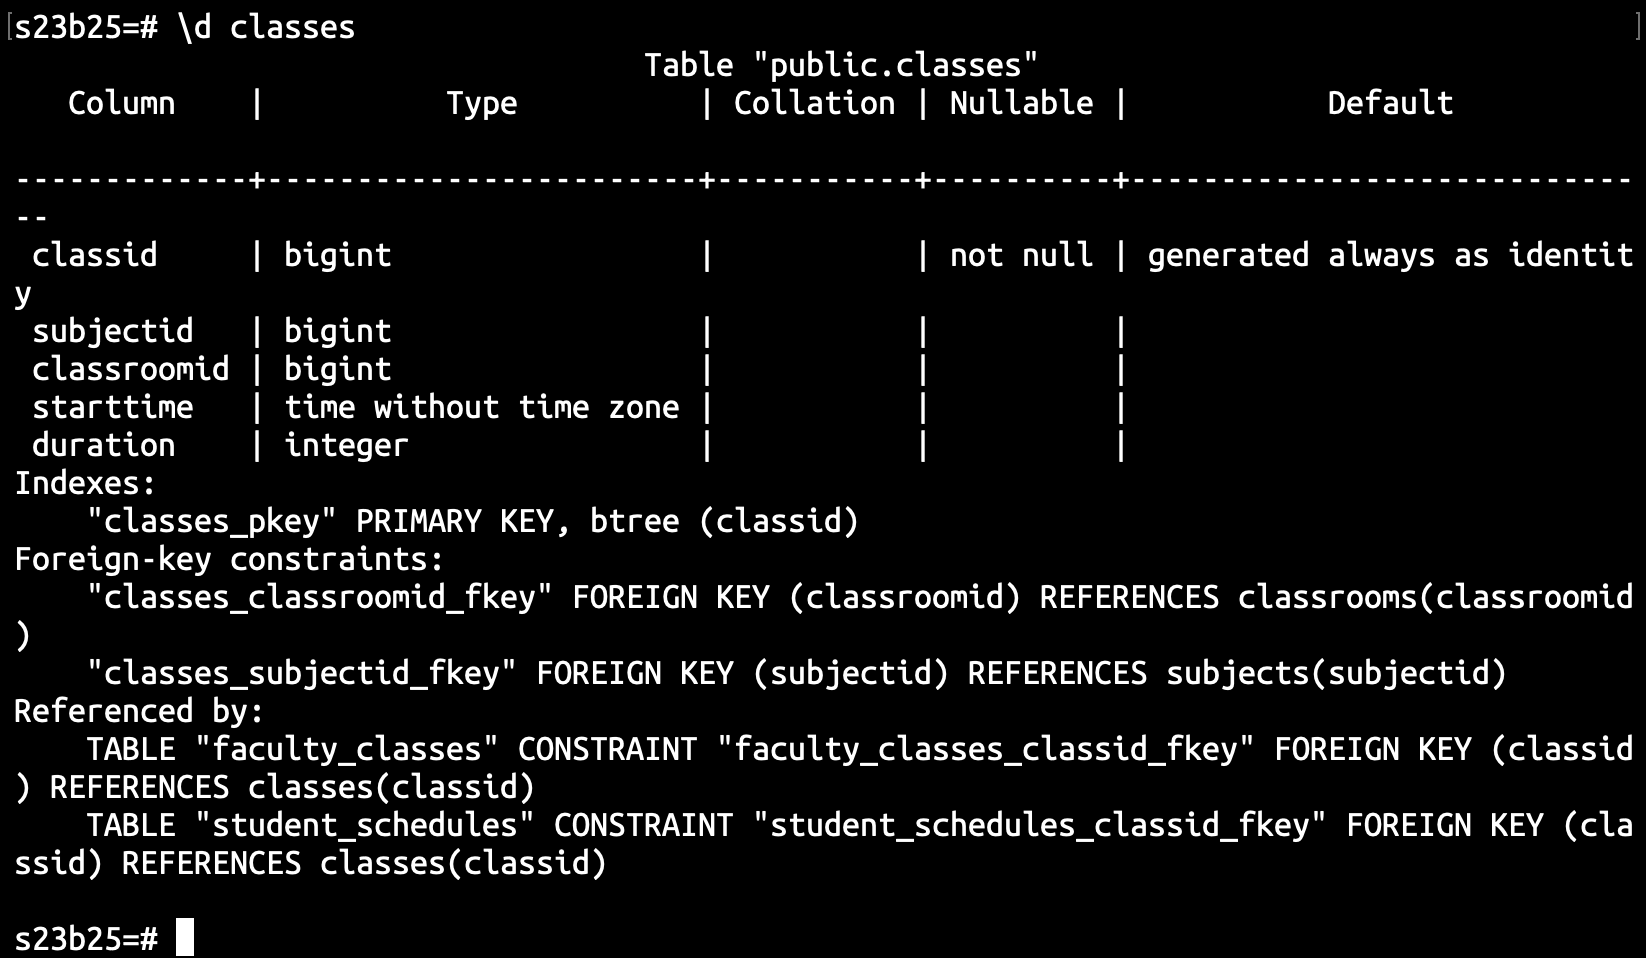
\includegraphics[width=\textwidth]{./o_9_classes.png}
\end{figure}

\subsubsection*{Faculty-Classes Table}
Query:
\begin{Verbatim}[frame=single,framerule=1pt,fontfamily=courier,fontsize=\small]
CREATE TABLE faculty_classes(
    staffID bigint REFERENCES staff (staffID),
    classID bigint REFERENCES classes (classID),
    PRIMARY KEY (staffID, classID)
);
\end{Verbatim}
\begin{figure}[h]
    \centering
    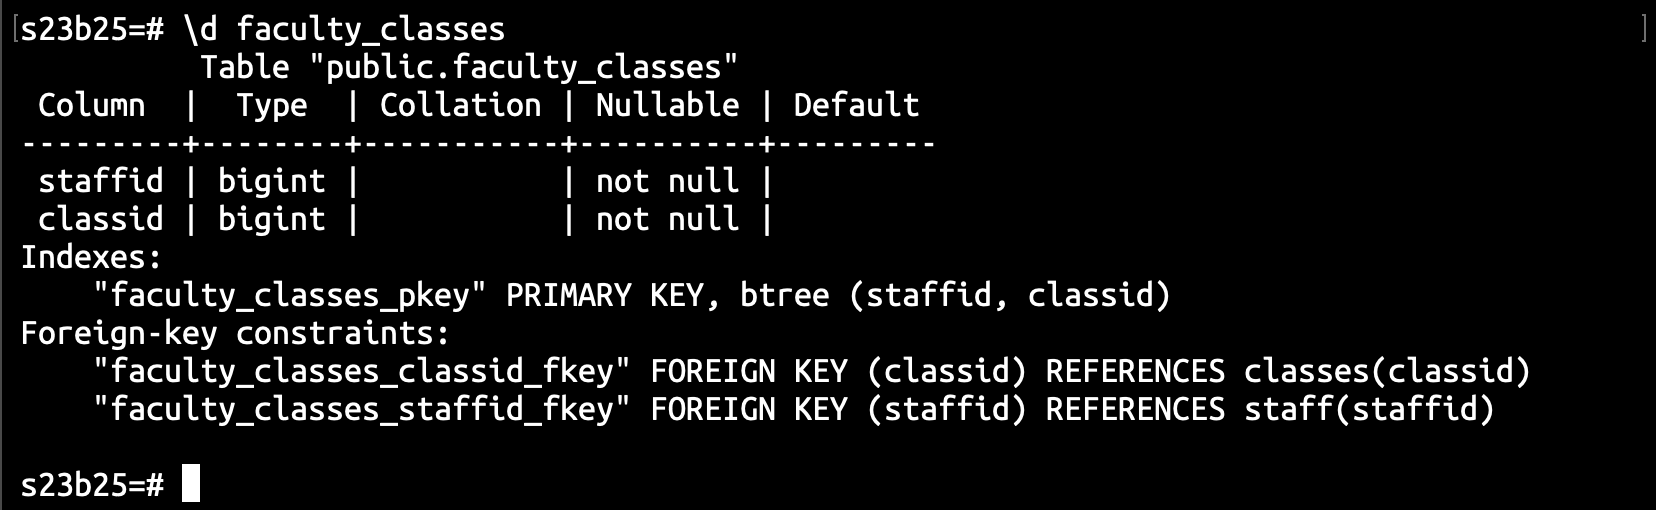
\includegraphics[width=\textwidth]{./o_10_faculty_classes.png}
\end{figure}

\subsubsection*{Students Table}
Query:
\begin{Verbatim}[frame=single,framerule=1pt,fontfamily=courier,fontsize=\small]
CREATE TABLE students(
    studentID bigint GENERATED ALWAYS AS IDENTITY PRIMARY KEY,
    studFirstName text,
    studLastName text,
    studStreetAdress text,
    studCity text,
    studState text,
    studZipCode int,
    studAreaCode int,
    studPhoneNumber text
);
\end{Verbatim}
\begin{figure}[h]
    \centering
    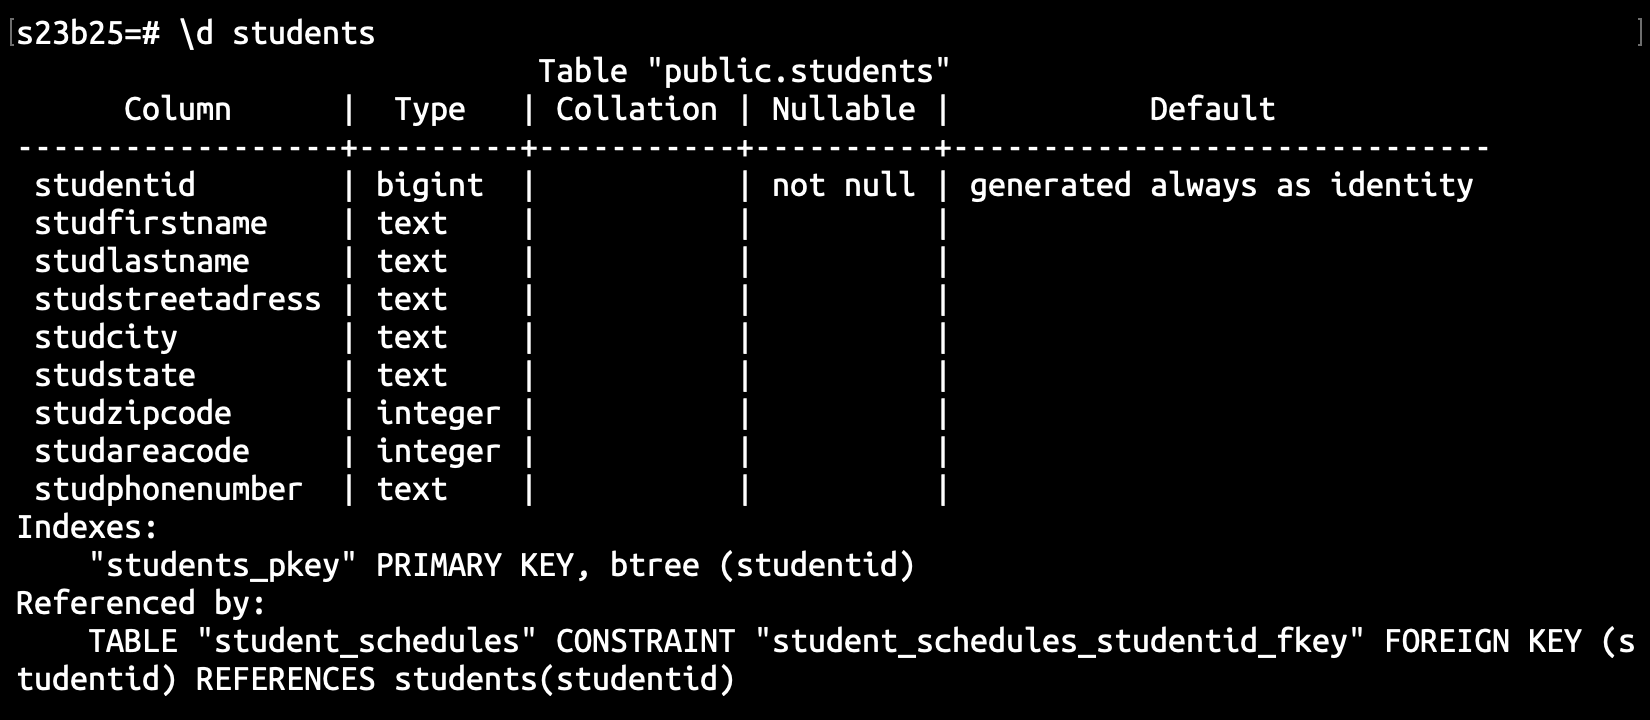
\includegraphics[width=\textwidth]{./o_11_students.png}
\end{figure}

\subsubsection*{Student-Class-Status Table}
Query:
\begin{Verbatim}[frame=single,framerule=1pt,fontfamily=courier,fontsize=\small]
CREATE TABLE student_class_status(
    classStatus bigint GENERATED ALWAYS AS IDENTITY PRIMARY KEY,
    classDescription text
);
\end{Verbatim}
\begin{figure}[h]
    \centering
    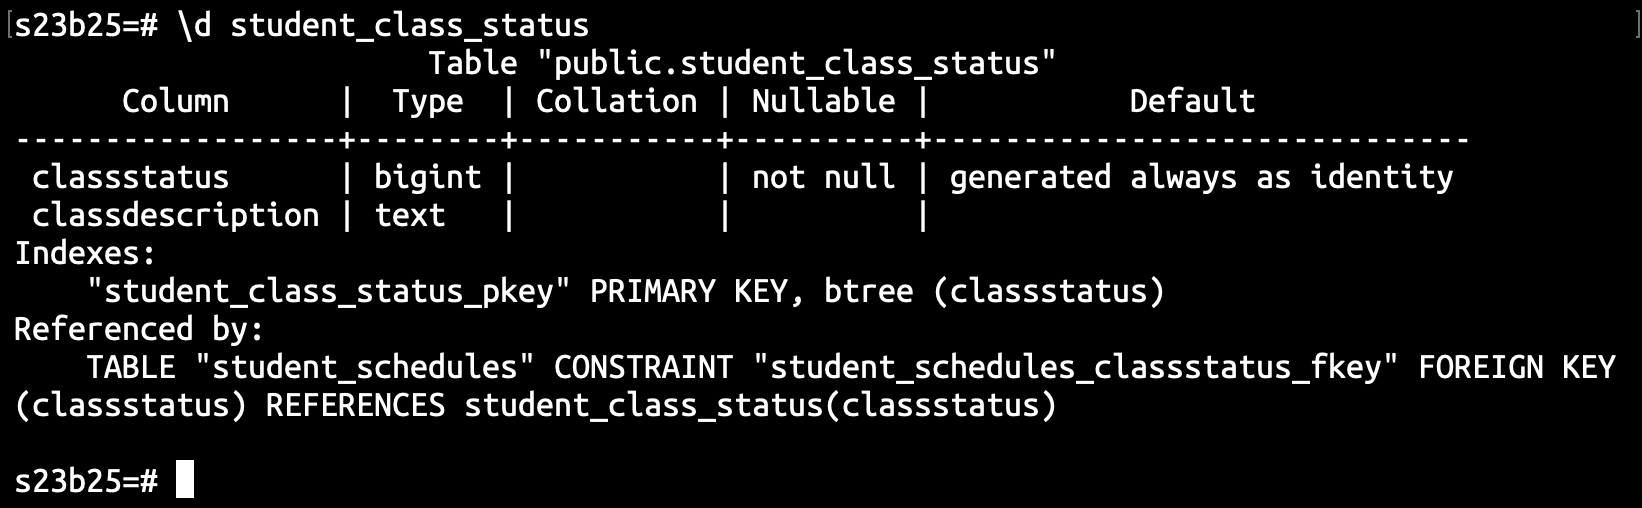
\includegraphics[width=\textwidth]{./o_12_student_class_status.png}
\end{figure}

\subsubsection*{Student-Schedules Table}
Query:
\begin{Verbatim}[frame=single,framerule=1pt,fontfamily=courier,fontsize=\small]
CREATE TABLE student_schedules(
    classID bigint REFERENCES classes (classID),
    studentID bigint REFERENCES students (studentID),
    classStatus bigint REFERENCES student_class_status (classStatus),
    grade int,
    PRIMARY KEY (classID, studentID)
);
\end{Verbatim}
\begin{figure}[h]
    \centering
    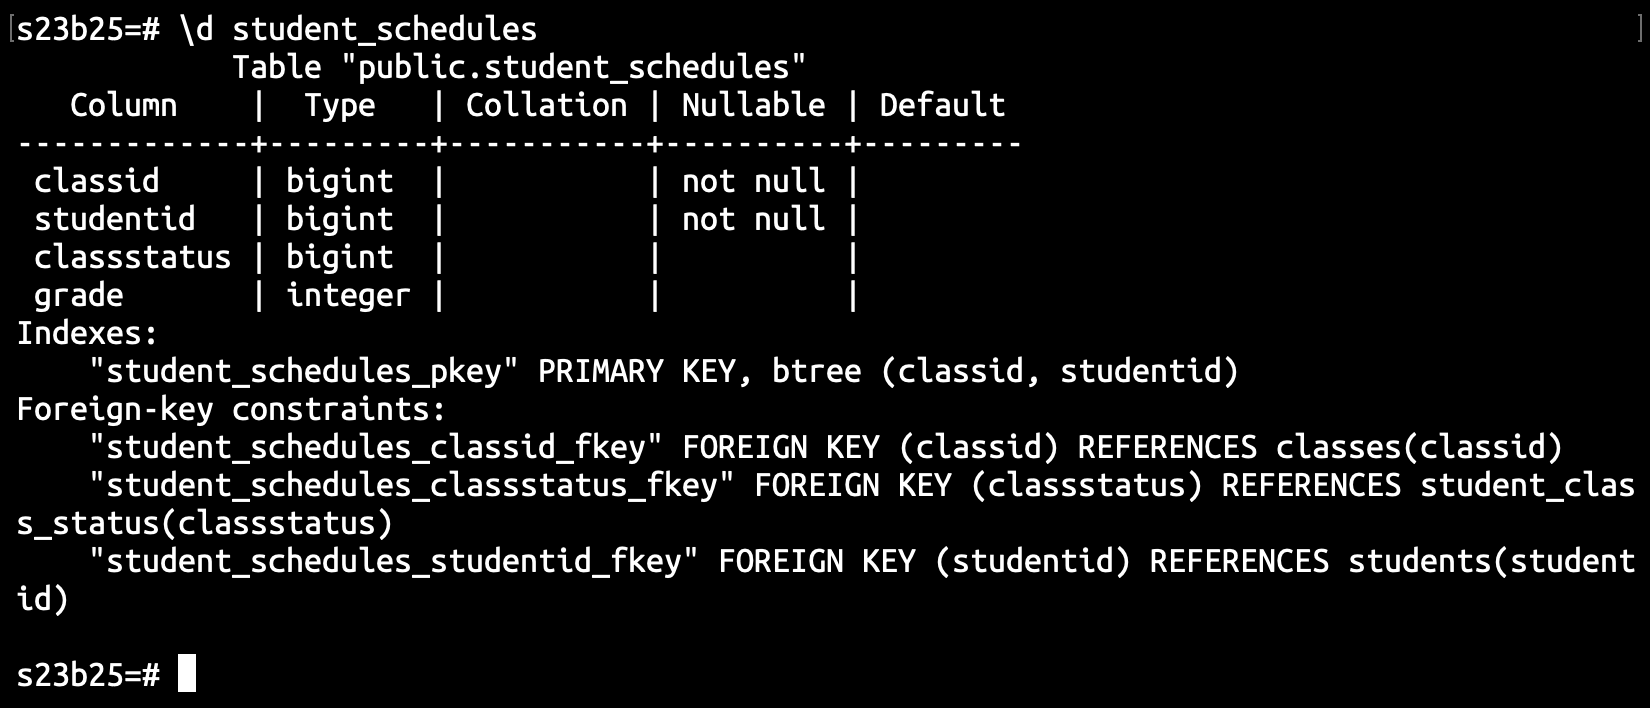
\includegraphics[width=\textwidth]{./o_13_student_schedules.png}
\end{figure}

\subsubsection*{Alter Staff Table}
Query:
\begin{Verbatim}[frame=single,framerule=1pt,fontfamily=courier,fontsize=\small]
ALTER TABLE staff RENAME COLUMN dateHired TO joiningDate;
\end{Verbatim}
\begin{figure}[h]
    \centering
    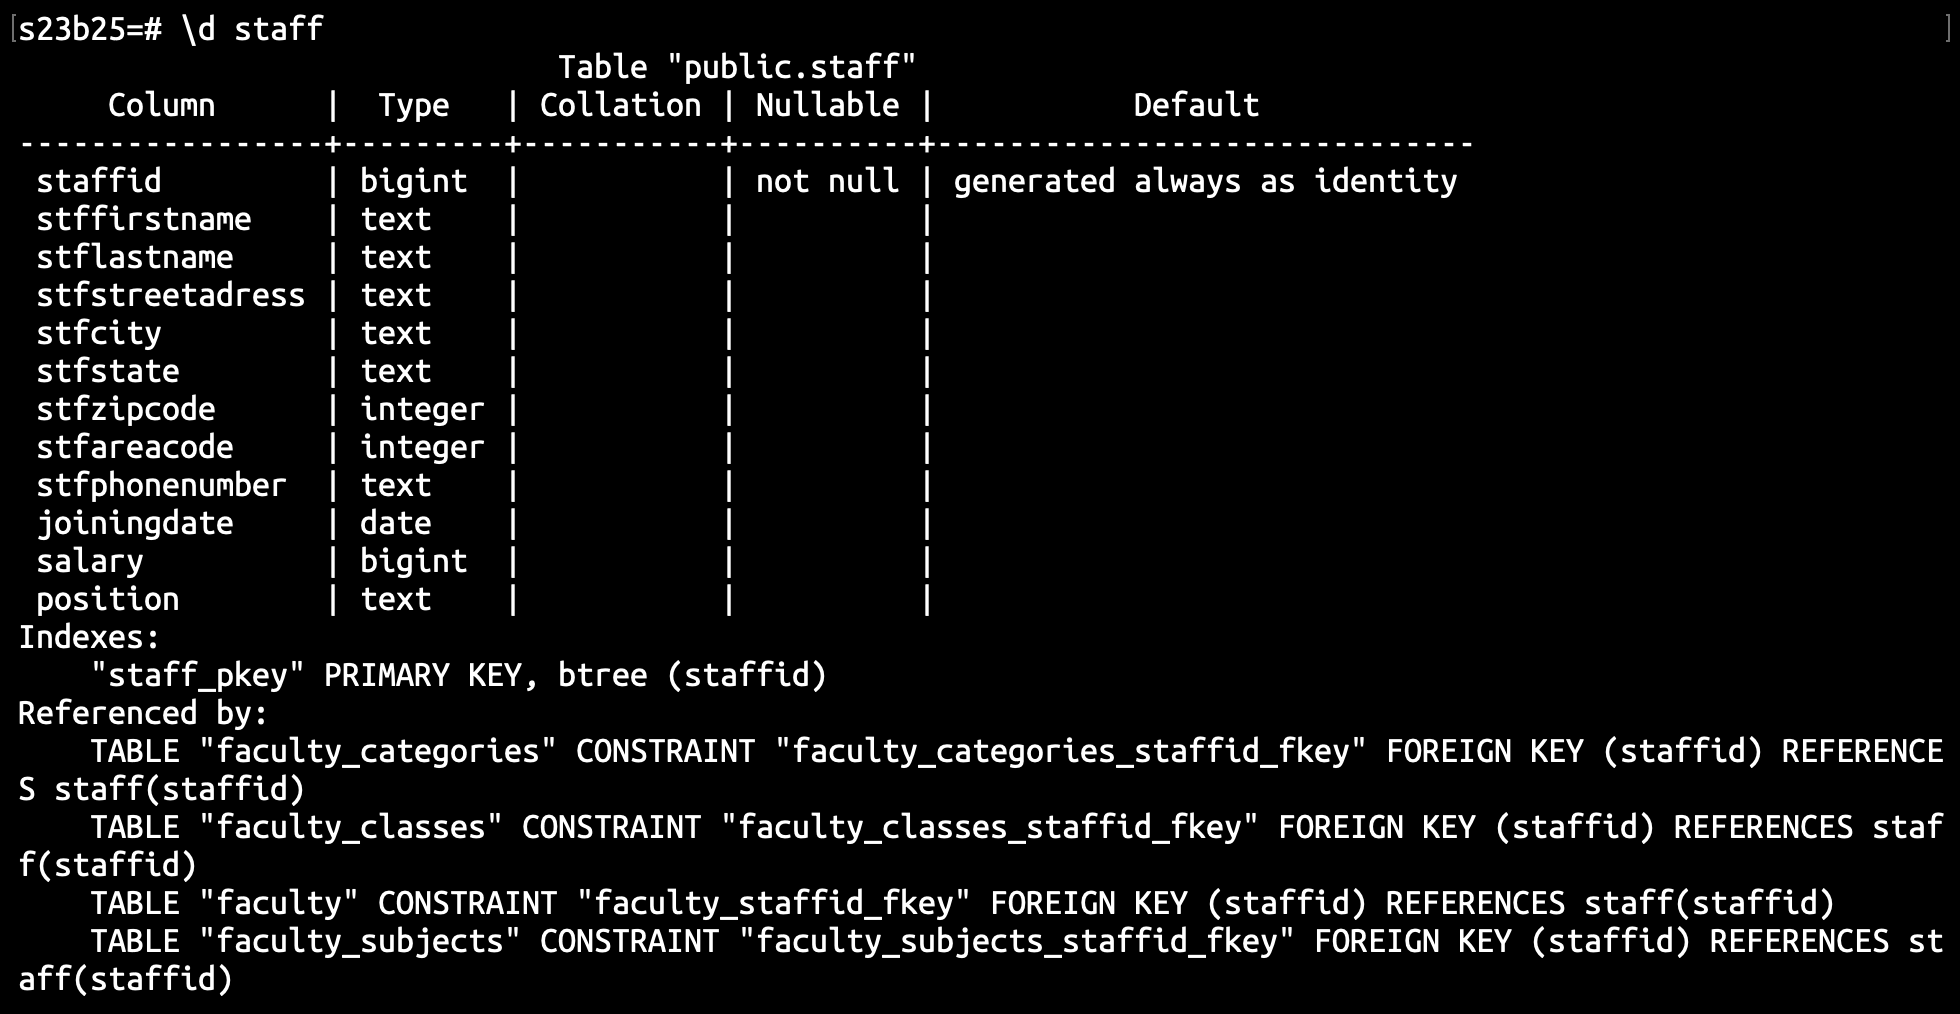
\includegraphics[width=\textwidth]{./o_14_alter_staff.png}
\end{figure}

\subsubsection*{Alter Subjects Table}
Query:
\begin{Verbatim}[frame=single,framerule=1pt,fontfamily=courier,fontsize=\small]
ALTER TABLE subjects DROP COLUMN subjectDescription;
\end{Verbatim}
\begin{figure}[h]
    \centering
    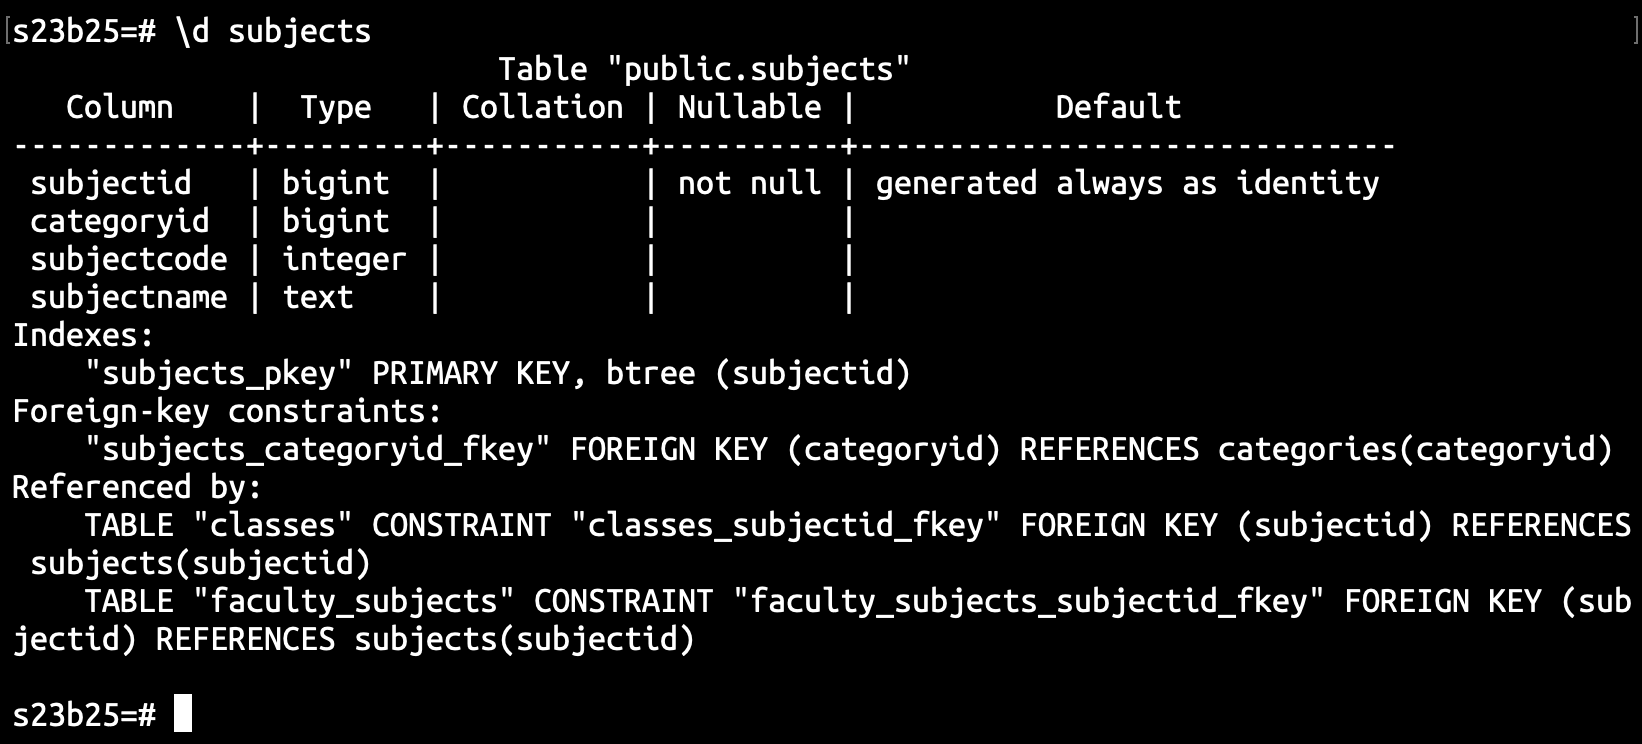
\includegraphics[width=\textwidth]{./o_15_alter_subjects.png}
\end{figure}

\end{document}
